\chapter{Widerstandsbestimmung (FT)}\label{s:widerstandsbestimmung}

Das Ziel dieser Arbeit ist es, festzustellen, ob die hybride aktive Str"omungsbeeinflussung von stumpfen K"orpern mittels gepulster Druckluftjets "uber zwei rotierende Coand\^{a}-Walzen mit kleiner Zahnzahl an der K"orperr"uckseite eine nennenswerte Widerstandsreduktion gegen"uber dem Fall ohne Beeinflussung erzielt. 
Dar"uber hinaus soll getestet werden, ob die periodische Aktuierung gegen"uber vorherigen Untersuchungen mit kontinuierlicher Ausblasung den Widerstand  st"arker senken kann und diese Form der Ausblasung effizienter als effizienter betrachtet werden kann.

Hierzu muss aus den Versuchsdaten einerseits die jeweiligen Widerstandswerte des K"orpers bestimmt werden. Andererseits ist es erforderlich, abzusch"atzen, ob diese Form der Str"omungsmodifikation unter dem Schlussstrich Energie einsparen kann oder f"ur die Aktuationsmechanismen m"oglicherweise sogar mehr Energie aufgewandt werden muss, als an Einsparung gewonnen werden kann.
Zus"atzlich ist es von Interesse zu bestimmen, wie gro\ss{} der Impulsstrom ist, der durch die Aktuation in die Str"omung eingebracht wird.

Die Gleichungen f"ur diese Zwecke sollen in diesem Kapitel hergeleitet und erl"autert werden.

\section{Bestimmung des Widerstands mittels des Impulssatzes}
\label{sec:WueberImpulssatz}
%Die nachfolgenden Ausf"uhrungen orientieren sich eng an  Hucho \cite{Hucho.2011}.
Die Widerstandskraft $W$ eines K"orpers innerhalb einer Unterschallstr"omung besteht im Wesentlichen aus den beiden Anteilen Reibungswiderstand und Druckwiderstand.
Bei schlanken K"orpern dominiert der Reibungswiderstand der aus Schubspannungen in der Grenzschicht der Geometrie resultiert. Bei stumpfen K"orpern hingegen dominiert fast ausnahmslos der Druckwiderstand, welcher seinen Ursprung wie bereits erw"ahnt in einer "uber den K"orper schwankenden Druckverteilung hat.


Der Widerstand $W$ eines stumpfen K"orpers innerhalb einer Str"omung macht sich als Impulsverlust derselben stromabw"arts bemerkbar. Diese gesuchte Gr"o\ss{}e kann somit bestimmt werden, in dem der Geschwindigkeitsverlauf der Str"omung im Nachlauf betrachtet und mittels des Impulssatzes ausgewertet wird. 

Der Widerstand des K"orpers selber l"asst sich finden, wenn ein Kontrollvolumen wie in \abb{fig:HuchoKV} um den K"orper gelegt und eine Impulsbilanz aufgestellt wird \cite{Hucho.2011}. Es wird im Folgenden vereinfacht von einer horizontalen, inkompressiblen 2D-Str"omung ausgegangen und der Impulssatz in x-Richtung

\begin{equation}
	\label{eq:impulssatz_allg}
	\rho \int_{(K)} v_x \, \mathrm{d}Q = F_{Kx} + F_{Px} + F_{Sx}
\end{equation}
betrachtet.

Die Dichte der umstr"omenden Luft wird hierbei mit $\rho$ bezeichnet.
Zudem entspricht in \glg{eq:impulssatz_allg} $F_{Kx}$ den angreifenden Volumenkr"aften, $F_{Px}$ der am freien Teil des Volumen angreifenden Oberfl"achenkr"afte (Druckkraft) und $F_{Sx}$ der St"utzkraft.

\begin{figure}[h]
	\centering
	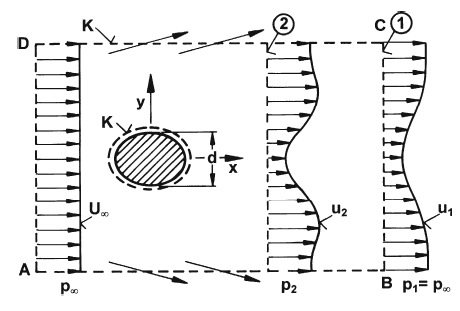
\includegraphics[width=0.5\textwidth]{KontrollvolumenHucho.png}
	\caption{Kontrollvolumen K um einen K"orper mit Geschwindigkeitsverteilungen u(x,y)~\cite{Hucho.2011}}
	\label{fig:HuchoKV}
\end{figure}

Die Volumenkraft $F_{Kx}$ kann dabei zu null gesetzt werden, da die Str"omung in Richtung x horizontal verl"auft und auch abgesehen von der Gewichtskraft keine anderen Volumenkr"afte wirken.

Wenn das Kontrollvolumen, wie es in \abb{fig:HuchoKV} zu sehen ist, weit genug ab vom K"orper gelegt ist, herrscht an den Begrenzungr"andern AD, BC, AB und DC der konstante Druck $p_{\infty}$.
Dies resultiert in einer Druckkraft $F_{Px} = 0$, da sich die Kr"afte an den R"andern aufheben.

Die St"utzkraft kann nun also dem Nettoimpulsfluss gleichgesetzt werden:
\begin{equation}
	\label{eq:nettoimpulsfluss}
	\rho \int_{(K)} \, v_x \, \mathrm{d}Q	= -\rho b \int u_1(u_{\infty} - u_1) \mathrm{d}y = F_{Sx}.	
\end{equation}
Hier ist $b$ die Breite des Modells senkrecht zur Zeichenebene und $U_{\infty}$ die Geschwindigkeit der umgest"orten Anstr"omung.

Die St"utzkraft des festen Teils des Kontrollvolumens - also des Stumpfk"orpers - h"angt mit dem Widerstand in der Form
\begin{equation}
	\label{eq:W=-F_Sx}
	W = - F_{Sx}
\end{equation}
zusammen. 
$W$ ist also gleich der St"utzkraft mit negativem Vorzeichen.

Daraus folgt der Ausdruck f"ur den Widerstand zu
\begin{center}
	\begin{equation}
		\label{eq:widerstand}
		W = \rho b \int u_{1} (u_{\infty}- u_{1}) \mathrm{d}y.
	\end{equation}
\end{center}

Der Widerstand l"asst sich f"ur bessere Vergleichbarkeit dimensionslos "uber den Widerstandsbeiwert $C_w$ ausdr"ucken. Dieser ist als 
\begin{center}
	\begin{equation}
		\label{eq:def-c_w}
		C_w = \frac{W}{\frac{\rho}{2}}\, U_{\infty}^2 \, bd
	\end{equation}
\end{center}
definiert.

Nach Einsetzen der Gleichung \ref{eq:widerstand} ergibt sich f"ur den Widerstandsbeiwert
\begin{equation}
	\label{eq:Bestimmungsgleichung C_w}
	C_w = \frac{2}{U_{\infty}^2 d} \int u_{1}(U_{\infty} - u_{1}) dy.
\end{equation}
%Die Integrationsgrenzen m"ussen an die vertikale Ausdehnung der Sonden am Messrechen im Nachlauf angepasst werden.	

Mit Hilfe dieser Formeln kann dann ein m"ogliche Reduktion des Widerstandsbeiwertes festgestellt werden.

Um den Geschwindigkeitsverlauf zu bestimmen, k"onnen mehrere Methoden angewandt werden, wobei im Rahmen dieser Arbeit die Geschwindigkeiten aus den dynamischen Dr"ucken ermittelt werden.

Der Messrechen im Nachlauf liefert hierzu statische Dr"ucke und Totaldr"ucke.

Da die Wirbel an der K"orperr"uckseite periodisch abl"osen, erwarten wir am Ort der Messungen - sprich im Nachlauf - ebenfalls periodische Druckschwankungen.
Von Relevanz f"ur die zu untersuchenden Fragestellung sind dabei allerdings nur die Mittelwerte dieser Messungen "uber mehrere Perioden.
Diese werden fu"r die einzelnen Sonden in der Form
\begin{center}	
	\begin{equation}
		\overline{p}=\sum_{i=0}^{n}\frac{p_i}{n}
	\end{equation}
\end{center}
zeitlich gemittelt.
Die Summe aller "uber einen Zeitraum genommenen Dr"ucke $p_i$ wird hierbei durch die Anzahl $n$ dieser Dr"ucke innerhalb dieses Zeitraums geteilt.
Diese Mittlung gleicht zudem in gewissem Ma\ss{}e das unvermeidbare Messrauschen aus.

"Uber den die Definition des dynamischen Drucks $q$ bzw. den Zusammenhang
\begin{center}
	\begin{equation}
		\label{geschwindigkeitsformel}
		u_{1}(y)= \sqrt{\frac{2}{\rho}(p_g - p_{\infty}) } = \sqrt{\frac{2}{\rho} q(y)}
	\end{equation}
\end{center}
l"asst sich wie oben beschrieben der Geschwindigkeitsverlauf aus den gemessenen Dr"ucken bestimmen und in \glg{eq:Bestimmungsgleichung C_w} einsetzen.

Wobei $u_{1}$ die Str"omungsgeschwindigkeit im Nachlauf in Abh"angigkeit der y-Koordinate und $q$ der gemessene dynamische Druck ist.

Diese gesamte Vorgehensweise zur Bestimmung des Widerstands ist legitim, wenn an der Messstelle im Nachlauf n"aherungsweise angenommen werden kann, dass der statische Druck wieder $p_\infty$ entspricht.In diesem Fall heben sich die Druckterme im Impulssatz auf  beiden Seiten des Kontrollvolumens gegenseitig auf.
Wird die Nachlaufdelle hingegen n"aher am K"orper gemessen, weicht der dort gemessene statische Druck von $p_{\infty}$ ab.
Solche Abweichungen lassen sich durch die messtechnische Anordnung nicht vermeiden - 
k"onnen nach \textit{B.M. Jones}, wie sie beispielsweise bei \textit{Schlichting} \cite{Schlichting.2001} zu finden ist, aber durch eine Korrektur ber"ucksichtigt werden.

Hierbei werden die Dr"ucke, die theoretisch an einem Querschnitt $1$ \abb{fig:HuchoKV} weit genug weg vom K"orper und somit von der statischen Druckabweichung herrschen, auf Dr"ucke zuruckgef"uhrt, die n"aher am K"orper tats"achlich gemessen werden.
Der neue Querschnitt, bei welchem die Messung stattfindet, erh"alt den Index $(2)$.

Der Widerstand in diesem Fall ergibt sich zu

\begin{equation}
	\label{eq:widerstand_korrigiert}
	W = 2b \int \sqrt{p_{t2} - p_2} \left(\sqrt{p_{t\infty} - p_{\infty}} - \sqrt{p_{t2} - p_{\infty}}\right) \mathrm{d} y_2 .
\end{equation}
Wobei $p_{t2}$ und $p_{t\infty}$ dem Totaldruck im Nachlaufquerschnitt bzw. dem Totaldruck der ungest"orten Anstr"omung entspricht.

F"ur den Widerstandsbeiwert erh"alt man

\begin{equation}
	\label{eq:C_w_korrigiert}
	C_w = 2 \int_{(2)} \sqrt{\frac{p_{t2} - p_2}{q_{\infty}}}
	\left(1 - \sqrt{\frac{p_{t2} - p_{\infty}}{q_{\infty}}}\right)  \mathrm{d}\left(\frac{y}{d}\right).
\end{equation}

Der Rechen, der die Druckverl"aufe liefert, muss zu diesem Zwecke so platziert werden, dass die Nachlaufdelle komplett aufgenommen wird. 


\section{Effizienzbetrachtung und Impulskoeffizient}

\subsection{Impulskoeffizient}
Der Impulskoeffizient $C_{\mu}$ wird als Ma\ss{} f"ur die Intensit"at der Ausblasung verwendet und ist im Falle von kontinuierlicher Ausblasung als 
\begin{equation}
	\label{eq: Def-momentum-coeff}
	C_{\mu} = 2 \,\frac{\dot{m}_{jet} \cdot U_{jet}}{\frac{1}{2}\rho_{\infty}\, \cdot U^2_{\infty} \cdot A_{ref}}
\end{equation}
definiert\cite{ElSayedM..2018}.
Dabei entspricht $\dot{m}_{jet}$ dem Massenstrom, der durch die Spalte ausgeblasen wird. $U_{jet}$ bezeichnet die Geschwindigkeit dieses Ausblasestroms.
$A_{ref}$ wiederum dient als Bezugsfl"ache. Im Falle des getesteten Stumpfk"orpers wird als $A_{ref}$ die projizierte Fl"ache der K"orperh"ohe verwendet, da beispielsweise der Druckwiderstand einen proportionalen Zusammenhang zu dieser f"ur stumpfe K"orper charakteristischen Fl"ache besitzt.  %\cite{Bilges.2018}

Die Periodizit"at der Ausblasung im Falle kann zus"atzlich im Impulskoeffizienten ber"ucksichtigt werden und f"uhrt letzendlich auf die Form \cite{Chabert.2014}
\begin{equation}
	\label{eq:momentum-coeff-oscill}
	\langle{C_{\mu}}\rangle = \frac{\rho_{jet}\langle{U^2_{jet}}\rangle \langle{A_{Spalt}}\rangle} {\frac{1}{2}\rho_{\infty}U^2_{\infty}A_{ref}}.	
\end{equation}
In \glg{eq:momentum-coeff-oscill} steht der $\langle{}\rangle$-Operator f"ur die jeweiligen zeitlichen Mittelwerte und $A_{Spalt}$ bezeichnet die Fl"ache des Ausblasespalts.

Da sowohl Plenumsdruck und somit auch die Ausblasegeschwindigkeit $U_{jet}$, als auch der Spaltquerschnitt "uber die Umdrehung der Walzen schwanken, m"ussen diese Einfl"usse wie in \glg{eq:eq:momentum-coeff-oscill} Eingang in die Formel f"ur $C_{\mu}$ im Falle der periodischen Aktuation finden.

F"ur das mit der Zeit variierende $A_{Spalt}$   wird die mittlere Spalth"ohe, die sich von dem Zeitpunkt der "Offnung des Spalts bis zu dem Zeitpunkt, an dem der Spalt gerade wieder geschlossen ist, ermittelt.  
Durch die Betrachtung des in \abschn{s:zahnform} dargestellten Spalth"ohenverlaufs ergibt sich ein $\langle{h_{Spalt,offen}}\rangle$ von ca. 0,18 \,mm.

Die mittlere Spalth"ohe "uber eine komplette Umdrehung ergibt sich durch die Multiplikation mit dem Tastgrad $\alpha$.


$U_{jet}$ muss im Falle der neu erprobten Testkonfiguration "uber die Plenumsdr"ucke berechnet werden.
Zun"achst werden aus den kontinuierlich ermittelten Messwerten f"ur die beiden Dr"ucke $p_{Plenum}$ mittlere Werte gebildet, die als Ausgangspunkt der Berechnung dienen.

Wir gehen weiterhin davon aus, dass der im Plenum vorhandene Druck vollst"andig in dynamischen Druck umgesetzt wird:

	\begin{equation}
	\label{eq:Annahme q}
		\langle{p_{Plenum}}\rangle = q_{jet}
	\end{equation}

%- wie in \abschn{sec:WueberImpulssatz} bereits erw"ahnt -%	
Da wir  von einer inkompressiblen Str"omung ausgehen, kann die Geschwindigkeit $\langle{U_{jet}}\rangle$ nun als
	
	\begin{equation}
	\label{eq:jetgeschwindigkeit}
		\langle{U_{jet}}\rangle = \sqrt{\frac{2 \langle{p_{Plenum}}\rangle}{\rho_{jet}}} = \sqrt{\frac{2 \langle{p_{Plenum}}\rangle}{\rho_{\infty}}}
	\end{equation}
ausgedr"uckt werden.

Dar"uber hinaus muss wie bereits erw"ahnt der Tastgrad (engl: Duty-Cycle) des Signals der Walzen $\alpha$  mitbetrachtet werden.
Bei den getesteten Walzen folgt f"ur 50 \% Tastgrad, dass die Ausblasung zumindest theoretisch exakt "uber die H"alfte einer Walzenumdrehung erfolgt.
%Daraus folgt f"ur den Impulskoeffizient mit Ber"ucksichtigung der Periodizit"at die Gleichung
%\begin{equation}
%	\label{eq:momentum-coeff-oscill-alpha}
%	\langle{C_{\mu}}\rangle = \alpha C_{\mu}
%\end{equation}	 

Wenn nun zus"atzlich bedacht wird, dass "uber zwei als gleich angen"aherte Spalte ausgeblasen wird, k"urzt sich dieser Faktor 2 genau mit dem Tastgrad und wir erhalten als modifizierten Impulskoeffizienten f"ur die zweite Konfiguration

	\begin{equation}
	\label{eq:momentum-coeff-oscill-final}
		\langle{C_{\mu}}\rangle = \frac{\rho_{jet}\langle{U^2_{jet}}\rangle \langle{A_{Spalt}}\rangle} {\frac{1}{2}\rho_{\infty}U^2_{\infty}A_{ref}} = \frac{2\langle{p_{Plenum}}\rangle \langle{h_{Spalt,offen}}\rangle \cdot b_{Spalt}} {\frac{1}{2}\rho_{\infty}U^2_{\infty}A_{ref}}
	\end{equation}

Mittels des Impulskoeffizienten kann die Effektivit"at der Ausblasung beschrieben werden.
Auch f"ur den Vergleich zwischen den untersuchten Walzenpaaren und mit den Daten von \citep{Bilges.2018} ist die Betrachtung des Impulskoeffizienten ma\ss{}geblich.

\subsection{Leistungskoeffizient und Leistungsrate}
Eine alleinige Betrachtung und ein Vergleich der $C_w$-Werte f"ur den Fall ohne Druckluftzuf"uhrung und rotierende Walzen, sowie den Fall mit aktiver Stro"mungsbeeinflussung ist nicht ausreichend, um eine vollst"andige Bewertung der unterschiedlichen Konfigurationen vorzunehmen.

Die durch eine Widerstandsreduktion bedingte Leistungseinsparung im Anwendungsfall k"onnte durchaus durch die extern aufzubringende Leistung f"ur Druckluft und Walzenrotation ausgeglichen oder "ubertroffen werden, sodass letztendlich zus"atzliche Energie aufgebracht und der Zweck der Anwendung verfehlt w"urde.

Ob diese Form der Str"omungsbeeinflussung also eine reale Netto-Leistungseinsparung zur Folge hat, muss folglich durch andere Kennzahlen quantifiziert werden.

Zun"achst verwenden wir f"ur die Effizienzbetrachtung eine Leistungsrate $PR$, die als 

\begin{equation}
	\label{eq:leistungsrate}
	PR = \frac{(W_0 - W)\cdot U_{\infty}}{\frac{1}{2} \dot{m_j} u_j^2 + \, P_M}
\end{equation}
eingef"uhrt wird.\cite{Freund.1994}

Der Z"ahler dr"uckt die eingesparte Widerstandsleistung des Falls mit aktiver Str"omungsbeeinflussung im Vergleich mit dem neutralen Fall aus.
Dieser Term quantifiziert somit, in welchem Umfang die Energiedissipation in der Str"omung im zweiten Versuch reduziert wurde.

Der Nenner hingegen repr"asentiert hingegen die Leistung welche dem Modell bzw. der Str"omung von externer Quelle zugef"uhrt werden muss, um den gew"unschten Effekt zu erzielen.

Der erste Summand $\frac{1}{2}\,\dot{m_j} u_j^2$ charakterisiert die kinetische Leistung der Druckluft-Jets, die durch die Spalte ausgeblasen werden. Diese Darstellung vernachl"assigt, dass die  Druckluftbeaufschlagung in den Leitungen Verluste mit sich tr"agt und auch der Kompressor selber keinen optimalen Wirkungsgrad besitzt. Somit handelt es sich bei diesem Term um die idealisierte Jet-Leistung.

Der zweite Summand $ P_M$ ist die kombinierte Motorleistung und tr"agt dem Zustand Rechnung, dass die rotierenden Walzen von zwei Elektromotoren angetrieben werden m"ussen. Diese sind f"ur den Ausgleich der an den Walzen auftretenden Widerst"anden wie Reibung an den Lagern zust"andig.
Diese Leistung wird mittels eines Leistungsmessger"ats ermittelt und manuell f"ur die Versuchsreihen notiert.


Des Weiteren wird als weitere Gr"o\ss{}e noch der Leistungskoeffizient $C_{Power}$ ben"otigt, welcher als
\begin{equation}
	\label{eq:def-powercoefficient}
	C_{Power,jet} = \frac{E_{jet}\dot{m}_{jet} + p_{jet}U_{jet}A_{jet} - (E_p\dot{m}_p + p_p U_p A_p)}{\frac{1}{2}\rho_{\infty}U^3_{\infty} A_{ref}}
\end{equation}

mit
\begin{equation}
	\label{eq:def-energieterm}
	E = c_vT + \frac{U^2}{2}
\end{equation}		
definiert ist.\cite{Hucho.2011}

Gr"o\ss{}en mit Index $p$ entsprechen dabei den Gr"o\ss{}en innerhalb des Plenums, in dem die Str"omung nicht kontrahiert wird.
Des Weiteren bezeichnet $c_v$ die spezifische W"armekapazit"at von Luft bei konstantem Volumen, $T$ die Temperatur der Luft und $U$ die Geschwindigkeit.

Dieser Koeffizient dr"uckt das Verh"altnis der aufzubringenden Leistung durch die Aktuation zur in der Antsr"omung vorhandenen Leistung aus.

Im Rahmen dieser Versuche wenden wir auf \glg{eq:def-powercoefficient} einige Vereinfachungen an. 

Zun"achst treffen wir die Annahmen, dass die Temperatur innerhalb des ausgeblasenen Luftstroms der Temperatur im Plenum entspricht

	\begin{equation}
	\label{eq:T-Vereinfachung}
		T_{jet} = T_{Plenum}
	\end{equation}

und wir n"aherungsweise davon ausgehen k"onnen, dass im Plenum keine Str"omungsgeschwindigkeit 

	\begin{equation}
	\label{eq:Up}
		U_{Plenum} = 0
	\end{equation}

vorliegt.

Des Weiteren nehmen wir, wie zuvor, an, dass die Str"omung inkompressibel ist und somit

	\begin{equation}
	\label{eq:Inkompressibilitaet}
		\rho_{jet} = \rho_{Plenum} = \rho_{\infty}
	\end{equation}
gilt.

Damit folgt f"ur den Leistungskoeffizienten der Ausblasung

	\begin{equation}
	\label{eq:CPowerJ vereinfacht}
		C_{Power,Jet} = \frac{\frac{1}{2}U^2_{jet} \cdot \dot{m}_{jet} \, + p_{jet}U_{jet}A_{jet}}{\frac{1}{2}\rho_{\infty}U^3_{\infty}A_{ref}}.
	\end{equation}

Im Falle periodischer Ausblasung muss anstatt $A_{jet}$ wieder $\langle{A_{jet}}\rangle$ verwendet werden.

Neben der Ausblasung wird auch der Aktuation durch die Walzen ein Leistungskoeffizient zugewiesen, welcher als
		\begin{equation}
		\label{eq:def-CPowerM}
			C_{Power,M} = \frac{P_M}{\frac{1}{2}\rho_{\infty}U^3_{\infty}A_{ref}}
		\end{equation}
		
definiert wird.
$P_M$ entspricht wieder der kombinierten Leistung der beiden Motoren.